\documentclass{sig-alternate}

\usepackage[utf8]{inputenc}

\usepackage[pdftex,urlcolor=black,colorlinks=true,linkcolor=black,citecolor=black]{hyperref}
\usepackage[capitalise,nameinlink]{cleveref}
\crefname{subsection}{Subsection}{Subsections}

\usepackage{graphicx}
\usepackage{caption}
\usepackage{subcaption}

% Better typography
\usepackage[activate]{microtype}

% Balance columns on last page
\usepackage{flushend}

% Todo macro
\usepackage{color}
\newcommand{\todo}[1]{\noindent\textcolor{red}{{\bf \{TODO} #1{\bf \}}}}

\begin{document}
%
% --- Author Metadata here ---
\conferenceinfo{SEXI}{'13 Rome, Italy}
\CopyrightYear{2013} % Allows default copyright year (20XX) to be over-ridden - IF NEED BE.
\crdata{}  % Allows default copyright data (0-89791-88-6/97/05) to be over-ridden - IF NEED BE.
% --- End of Author Metadata ---

\title{Identifying VHS Recording Artifacts\\
in the Age of Online Video Platforms}
\subtitle{[Position Paper]
}
%
% You need the command \numberofauthors to handle the 'placement
% and alignment' of the authors beneath the title.
%
% For aesthetic reasons, we recommend 'three authors at a time'
% i.e. three 'name/affiliation blocks' be placed beneath the title.
%
% NOTE: You are NOT restricted in how many 'rows' of
% "name/affiliations" may appear. We just ask that you restrict
% the number of 'columns' to three.
%
% Because of the available 'opening page real-estate'
% we ask you to refrain from putting more than six authors
% (two rows with three columns) beneath the article title.
% More than six makes the first-page appear very cluttered indeed.
%
% Use the \alignauthor commands to handle the names
% and affiliations for an 'aesthetic maximum' of six authors.
% Add names, affiliations, addresses for
% the seventh etc. author(s) as the argument for the
% \additionalauthors command.
% These 'additional authors' will be output/set for you
% without further effort on your part as the last section in
% the body of your article BEFORE References or any Appendices.

\numberofauthors{5}
\author{
\alignauthor
Thomas Steiner\\
       \affaddr{Univ. Politècnica de Catalunya}\\
       \affaddr{Department LSI}\\
       \affaddr{Barcelona, Spain}\\
       \email{tsteiner@lsi.upc.edu}
% 2nd. author
\alignauthor
Seth van Hooland\\
       \affaddr{Université Libre de Bruxelles}\\
       \affaddr{Information and C.S. Dept.}\\
       \affaddr{Brussels, Belgium}\\
       \email{svhooland@ulb.ac.be}
% 3rd. author
\alignauthor
Ruben Verborgh\\
       \affaddr{Ghent University}\\
       \affaddr{iMinds -- Multimedia Lab}\\
       \affaddr{Ghent, Belgium}\\
       \email{ruben.verborgh@ugent.be}
\and  % use '\and' if you need 'another row' of author names
% 4th. author
\alignauthor
Joseph Tennis\\
       \affaddr{Information School}\\
       \affaddr{University of Washington}\\
       \affaddr{Washington, D.C., USA}\\
       \email{jtennis@uw.edu}
% 5th. author
\alignauthor
Rik Van de Walle\\
       \affaddr{Ghent University}\\
       \affaddr{iMinds -- Multimedia Lab}\\
       \affaddr{Ghent, Belgium}\\
       \email{rik.vandewalle@ugent.be}
}

\maketitle
\begin{abstract}
In this position paper, we describe how analogue recording artifacts
stemming from digitalized {\scshape vhs} tapes such as
grainy noises, ghosting, or synchronization issues
can be identified at Web-scale via crowdsourcing
in order to identify adult content digitalized by amateurs.
\end{abstract}

% A category with the (minimum) three required fields
\category{H.4}{Information Systems Applications}{Miscellaneous}
%A category including the fourth, optional field follows...
%\category{D.2.8}{Software Engineering}{Metrics}[complexity measures, performance measures]

%\terms{Theory}

\keywords{Amateur Video Digitalization, Video Home System, Long Tail, Online Video Platforms}

\section{Introduction}

Online adult video is one of the fastest growing Internet industries
as recent statistics of a~large meta search engine for adult content
show\footnote{\url{http://www.pornwatchers.com/content/statistics11-2012/}}.
Since its launch in 2006, the search engine has indexed
the amount of overall 735,000 videos at a~growth rate of 22,000 videos per month
with overall 93 billion views.
Over this period, 158 million user ratings were collected.
It becomes evident that efficient search, recommendation, and
navigation capabilities are required in order to use
adult video platforms in a~meaningful way.
Online adult video platforms typically allow their users
(i)~to search for content based on full-text query terms
that are matched against textual descriptions
of the video like its title or description,
or (ii)~to browse the archive of a~platform by category or channel,
usually based on video tags.
Users are presented a~top-$n$ ranked list of videos
that match a~given category
or query term, ranked by criteria such as
\emph{relevancy}, \emph{view count},
\emph{user rating}, or \emph{upload date}.
The default ranking criterion normally is
\emph{relevancy}---a~platform-specific \emph{black box} concept.
Advanced and frequently returning power-users
may prefer more transparent and traceable ranking criteria
such as the popularity-based \emph{view count}
and \emph{user rating}, or the stack-based
{\scshape lifo} (last in, first out) ranking criterion \emph{upload date}.

In this position paper, we suggest a~computer vision-based
approach to automatically identify {\scshape vhs} adult content
that has been digitalized in a~non-professional manner.
This type of niche adult content is characterized by
analogue recording artifacts stemming from {\scshape vhs} tapes.
Common issues include
ghosting, brightness and color channel interferences,
chaotic line shift at the end of frames (\autoref{fig:ghosting}),
and wide horizontal noise strips (\autoref{fig:distortion}).

\begin{figure}[b!]
  \centering
  \begin{subfigure}[b]{0.45\linewidth}
    \centering
    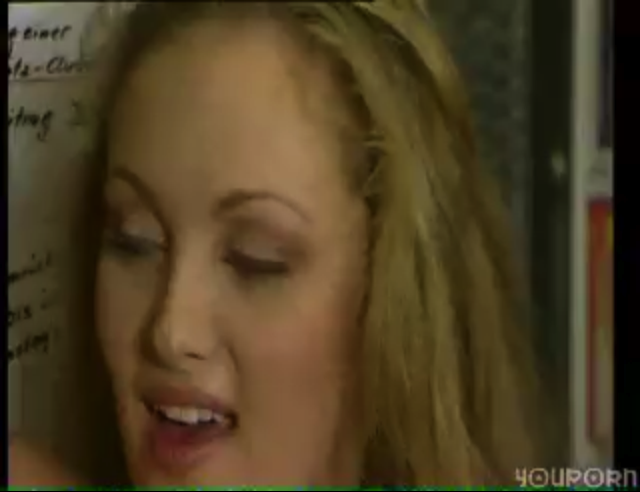
\includegraphics[width=\textwidth]{lineshift.png}
    \caption{Chaotic line shift at the bottom of frames (green)}
     \label{fig:ghosting}
  \end{subfigure}
  \begin{subfigure}[b]{0.45\linewidth}
    \centering
    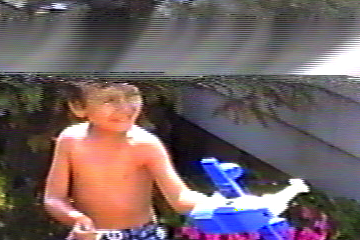
\includegraphics[width=\textwidth]{distortion.png}
    \caption{Wide horizontal noise strip distortions}
     \label{fig:distortion}
  \end{subfigure}
  \label{fig:artifacts}
  \caption{Typical {\scshape vhs} artifacts and distortions after amateurish digitalization.}
\end{figure}

\section{Problem Statement}

The publication of online content produced by
\emph{amateurs}, or non-professionals, has
received a~substantial amount of attention.
This position paper raises the question: to what extent
can the identification of content as {\scshape vhs adult content digitalized by amateurs}
offer a~useful parameter?
Exploiting the fact that an individual invested time and resources for the
digitalization of content from a~{\scshape vhs} tape can hold a~unique value
both for information retrieval and research purposes.
Especially in the context of the long tail of niche content,
automatically identifying {\scshape vhs adult content digitalized by amateurs}
can help identify more quickly unique content items.

Uploaders of this type of content occasionally add tags
such as ``vintage'' or ``retro'' but these practices are not standardized and sparse.
On the aforementioned adult content platform, out of overall 735,000 videos,
there were 23.427 tagged as ``vintage'', 95 as ``vhs'',
and only 50 as ``vintage'' \emph{and} ``vhs''.
Automated means to aggregate this type of content are needed
and therefore this position paper proposes a~scalable, crowdsourced way
to identify adult content digitalized by amateurs.

\section{Proposed Methodology}

In~\cite{steiner2011crowdsourcing}, we have introduced
a~generic crowdsourcing framework for the automatic and scalable
annotation of {\scshape html5} video.
While a~user watches a~video, the framework in the background
unobtrusively annotates it, \emph{e.g.}, as demonstrated
in the concrete case, to extract events.
The annotation framework being generic,
we can imagine a~video denoising algorithm
as presented by Yang in~\cite{yang2009videonoise}
being applied to a~video that is currently played
to detect if it suffers from {\scshape vhs} artifacts.
Over time, \emph{individual} users watching low quality digitalized videos
create enough signals to eventually filter out the corpus of
content digitalized by amateurs.

\section{Conclusion}

In this position paper, we have presented a~crowdsourced,
scalable approach to detect {\scshape vhs} digitalization artifacts,
where users by watching videos do useful work such as
detecting {\scshape vhs} artifacts as a~by-product of viewing,
and thus over time allowing video platforms to identify
a~specific type of niche content for further processing or filtering purposes.

\bibliographystyle{splncs03}
\bibliography{references}

\end{document}
